\documentclass[tikz,border=8pt]{standalone}
% Shared look for every TikZ diagram. Load with \input{../../tools/tikz-style.tex}
\usepackage[T1]{fontenc}
\usepackage{lmodern}
\renewcommand{\sfdefault}{lmr}  % diagrams use the same serif as the text
\usetikzlibrary{arrows.meta, positioning, shapes.geometric, calc, fit, backgrounds}
\definecolor{cblue}{HTML}{4C78A8}
\definecolor{corange}{HTML}{F58518}
\definecolor{cgreen}{HTML}{54A24B}
\definecolor{cred}{HTML}{E45756}
\definecolor{cpurple}{HTML}{B279A2}
\definecolor{cgrey}{HTML}{6B6B6B}
\tikzset{
  every picture/.style={font=\sffamily, line width=1.2pt},
  box/.style={draw=#1, fill=#1!12, rounded corners=4pt, align=center, inner sep=7pt, minimum height=1.1cm},
  box/.default=cgrey,
  arrow/.style={-{Stealth[length=3mm]}, draw=cgrey, line width=1.4pt},
  title/.style={font=\sffamily\bfseries\Large},
  note/.style={font=\sffamily\small, text=cgrey, align=center},
}
\AtBeginDocument{\hyphenpenalty=10000 \exhyphenpenalty=10000}

\begin{document}
% Section 3: the two branches. Descriptive statistics summarises the data in hand (the 891 Titanic fares); inferential
% statistics reasons from a sample to a population we cannot fully observe (the salary survey of section 4).
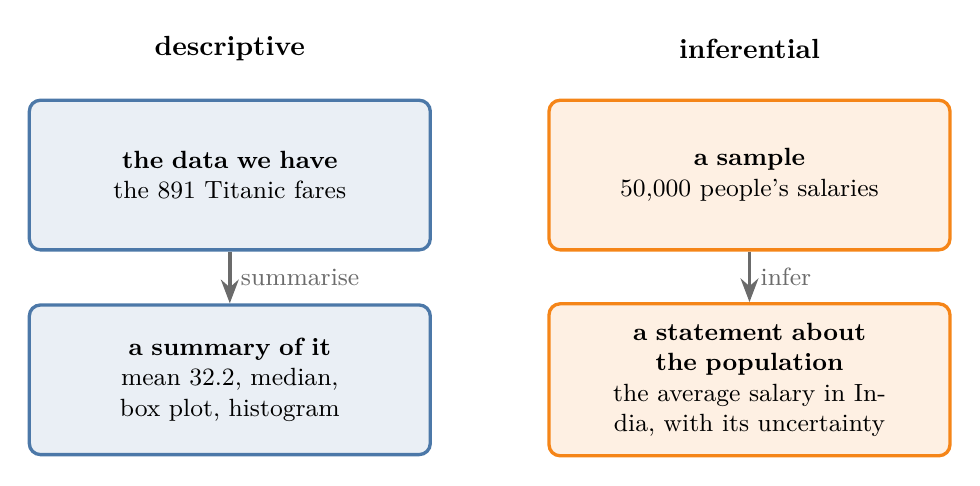
\begin{tikzpicture}[b/.style={box=#1, text width=4.6cm, minimum height=1.9cm, align=center, font=\sffamily\small}]
  \node[title, font=\sffamily\bfseries] at (0, 1.6) {descriptive};
  \node[b=cblue] (d1) at (0, 0) {\textbf{the data we have}\\the 891 Titanic fares};
  \node[b=cblue] (d2) at (0, -2.6) {\textbf{a summary of it}\\mean 32.2, median, box plot, histogram};
  \draw[arrow] (d1) -- node[right, note] {summarise} (d2);
  \node[title, font=\sffamily\bfseries] at (6.6, 1.6) {inferential};
  \node[b=corange] (i1) at (6.6, 0) {\textbf{a sample}\\50,000 people's salaries};
  \node[b=corange] (i2) at (6.6, -2.6) {\textbf{a statement about the population}\\the average salary in India, with its uncertainty};
  \draw[arrow] (i1) -- node[right, note] {infer} (i2);
\end{tikzpicture}
\end{document}
